% 5. projekt do předmětu ITY
% Autor: Jan Havlín, 1BIT, xhavli47@stud.fit.vutbr.cz
% Datum: 28. 4. 2018
% Popis: Prezentace na konečné automaty

\documentclass{beamer}
\usepackage[czech]{babel}
\usepackage[utf8]{inputenc}
\usepackage[T1]{fontenc}
\usepackage{graphics}

\usetheme{Rochester}

\title{Konečné automaty}
\author{Jan Havlín}
\institute
{Fakulta informačních technologií\\
Vysoké učení technické v~Brně}
\date{\today}

\begin{document}

\begin{frame}
  \titlepage
\end{frame}

\begin{frame}{Formální definice}
Konečný automat je definován jako uspořádaná pětice $\left(S, \Sigma, \sigma, s, A \right)$, kde:
\begin{itemize}
	\item{$S$ je konečná neprázdná množina \emph{stavů}.}
	\item{$\Sigma$ je konečná neprázdná množina vstupních symbolů, nazývaná \emph{abeceda}.}
	\item{$\sigma$ je tzv. \emph{přechodová funkce} (též \emph{přechodová tabulka}), popisující pravidla přechodů mezi stavy. Může mít buď podobu $S \times \Sigma \rightarrow S$ (deterministický automat), nebo $S \times \{\Sigma \cup \epsilon \rightarrow P(S)$ (nedeterministický automat), viz níže.}
	\item{$s$ je \emph{počáteční stav}, $s \in S$.}
	\item{$A$ je množina \emph{přijímajících stavů}, $A \subseteq S$.}
\end{itemize}
\end{frame}


\begin{frame}{Popis činnosti automatu}
\begin{itemize}
	\item{Na počátku se automat nachází v~počátečním stavu.}
	\item{V~každém kroku přečte jeden symbol ze vstupu.}
	\item{Přejde do stavu, který je dán hodnotou v~přechodové tabulce.}
	\item{Opakuje se čtení symbolu a~přechod stavu.}
	\item{Podle toho, zda automat skončí ve stavu patřícím do množiny přijímajících stavů platí, že automat buď vstup \emph{přijal}, nebo \emph{nepřijal}.}
\end{itemize}
\end{frame}

\begin{frame}{Příklad konečného automatu}
Jako příklad si uvedeme následující konečný automat:
\begin{itemize}
	\item{$S = (S_0, S_1, S_2$)}
	\item{$\Sigma = (0, 1)$}
	\item{$\sigma$ viz tabulka:
	\begin{table}[h]
	\begin{tabular}{|c|c|c|}
	\hline
	\textbf{stav}  & \textbf{0} & \textbf{1} \\ \hline
	$S_0$ & $S_0$      & $S_1$      \\ \hline
	$S_1$ & $S_2$      & $S_0$      \\ \hline
	$S_2$ & $S_1$      & $S_2$      \\ \hline
	\end{tabular}
	\end{table}
	}

	\item{$s = S_0$}
	\item{$A = \{S_0\}$}
\end{itemize}
\end{frame}

\begin{frame}{Grafické znázornění}
Pro popis konečného automatu se obvykle používá grafické znázornění.
	\begin{figure}[h]
	\begin{center}
	\scalebox{1.2}{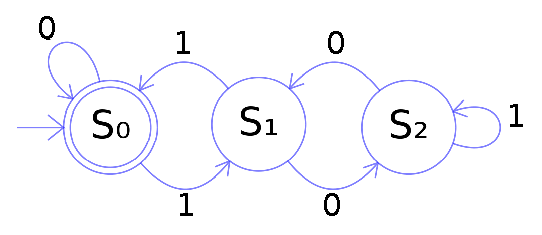
\includegraphics{automat.eps}}
	\end{center}
	\end{figure}
\end{frame}

\begin{frame}{Zpracování vstupu}
Při vstupu \texttt{1011} bude předchozí automat postupovat takto:
\begin{itemize}
    \item {Automat je ve stavu $S_0$.}
    \item {Na vstup přijde \texttt{1}, automat přejde do stavu $S_1$.}
    \item {Na vstup přijde \texttt{0}, automat přejde do stavu $S_2$.}
    \item {Na vstup přijde \texttt{1}, zůstane ve stavu $S_2$.}
    \item {Na vstup přijde \texttt{1}, zůstane ve stavu $S_2$.}
\end{itemize}

Stav $S_2$ \emph{nepatří} do množiny $A$, tudíž automat vstup \texttt{1011} \emph{nepřijal}.\\ \bigskip
Tento konečný automat přijímá regulární jazyk řetězců, které vyjadřují binární číslo dělitelné třemi.
\end{frame}

\begin{frame}{Použité zdroje}
\begin{itemize}
    \item{Konečný automat \\ 
    \url{https://cs.wikipedia.org/wiki/Kone\%C4\%8Dn\%C3\%BD_automat}}
\end{itemize}
\end{frame}
\end{document}
